\chapter{Электростатический подвес} \label{chapt1}


\section{Принципы построения электростатических подвесов} \label{sect1_1}

Электростатический подвес представляет собой устройство, удерживающее твердое тело во взвешенном состоянии за счет действия электрических сил, создаваемых системой из конечного количества электродов. Как правило, твердое тело является проводником, а в межэлектродном пространстве поддерживается вакуум.

Как известно \cite{Tamm}, заряд в проводящем теле, находящемся в электрическом поле, распределен таким образом, чтобы внутри тела электрическое поле отсутствовало. Таким образом, на проводник в электрическом поле действуют только поверхностные силы, которые направлены по внешней нормали к поверхности проводника. Величина этих сил невелика, поэтому для увеличения удерживающей силы необходимо увеличивать напряженность. При этом максимальная напряженность поля ограничена электрическим пробоем вакуумного промежутка между поверхностями тела и электродов, значение которого зависит от чистоты проводника, материала проводника, величины достигнутого вакуума и пр. Малость электрических сил вынуждает производить электростатические подвесы с малым межэлектродным промежутком, что влечет за собой необходимость сложного высокоточного производства. Например, сферический  электростатический высокоточный гироскоп ЭВГ имеет диаметр ротора порядка 1-2 см, расстояния между ротором и электродом измеряются десятками и сотнями микрометров \cite{Electropribor}.

\subsection{Обоснованность применения теории электростатики} \label{sect1_1_1}

Твердое тело в электростатическом подвесе находится в вакуумированной полости, ограниченной конечным числом проводящих электродов. Строго говоря, электрическое поле, потенциалы на электродах которого являются функциями от фазовых координат и времени, не является электростатическим. Тем не менее, можно показать, что выполняются условия квазистационарности, которые сводятся к требованию \cite{Tamm}:
\[
T^* \gg \tau,
\]
где $T^*$ – характерное время в движении твердого тела, $\tau = L^*/c$ – время запаздывания, $L^*$ – характерный размер системы, $c$ – скорость света. При $T^* \sim 10^{-3}$ с, $L^* \sim 10^{-3}$ см время $\tau \sim 0.3 \cdot 10^{-9}$ с, $\tau/T^* \sim 10^{-6}$.
Поэтому, пренебрегая запаздыванием системы, можем с приемлемой для практики точностью считать поле стационарным и в каждый момент времени решать задачу электростатики \cite{Martynenko}.

\subsection{Краткое описание основного объекта исследования, сферического ротора в электростатическом подвесе} \label{sect1_1_2}

!!!Из книги электроприбора или удалить!!!


\section{Обзор технических элементов, в которых находит свое применение электростатический подвес} \label{sect1_2}
Отсутствие трения является главным достоинством неконтактных подвесов, что позволяет создавать практически «вечные» подшипники, не имеющие проблем износа, шума и ограничений по скорости вращения. Отсюда вытекает множество прикладных решений, построенных на основе таких подвесов. Наиболее распространены неконтактные подвесы в навигации (на рисунке \ref{img:sphere_suspension_photo} – гироскоп с электростатическим подвесом), космической и транспортной отраслях.
Появление электростатических подвесов дало мощный толчок развитию гироскопической техники, неожиданно открылись совершенно новые интересные задачи \cite{Electropribor}.

\begin{figure}[ht] 
  \centering
  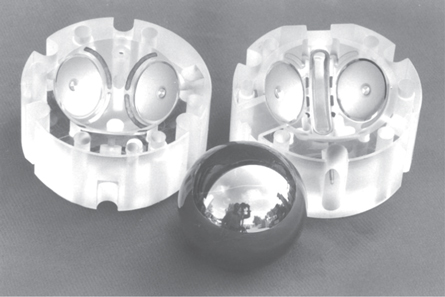
\includegraphics [scale=0.7] {sphere_suspension_photo}
  \caption{Сферический гироскоп с электростатическим подвесом. Фотография ротора и корпуса}
  \label{img:sphere_suspension_photo}
\end{figure}

%\newpage
%============================================================================================================================


%\newpage
%============================================================================================================================
